\documentclass[border=6pt]{standalone}
\usepackage{tikz}
\usetikzlibrary{arrows.meta,positioning,calc,shapes.geometric,fit,backgrounds,patterns,matrix,decorations.pathreplacing}
\begin{document}
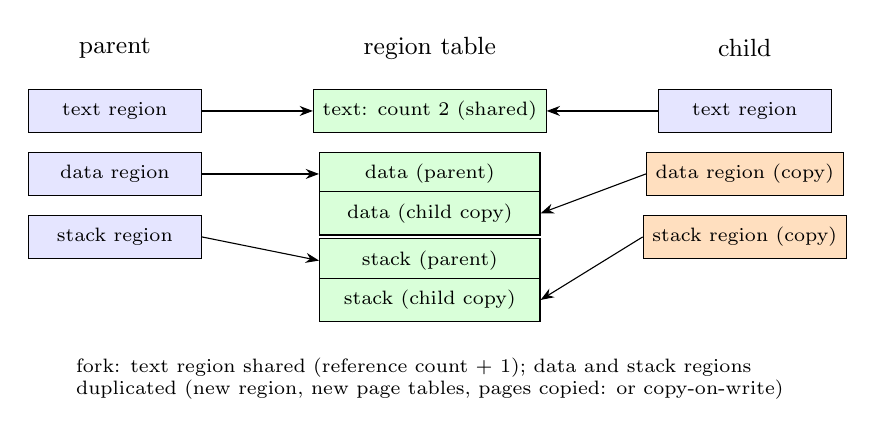
\begin{tikzpicture}[>=Stealth,font=\small]
\tikzstyle{c}=[draw,minimum height=0.55cm,minimum width=2.2cm,font=\scriptsize]
\node[font=\small] at (0,2.6) {parent};
\node[font=\small] at (4,2.6) {region table};
\node[font=\small] at (8,2.6) {child};
\node[c,fill=blue!10] (pt) at (0,1.8) {text region}; \node[c,fill=blue!10] (pd) at (0,1.0) {data region}; \node[c,fill=blue!10] (ps) at (0,0.2) {stack region};
\node[c,fill=blue!10] (ct) at (8,1.8) {text region}; \node[c,fill=orange!25] (cd) at (8,1.0) {data region (copy)}; \node[c,fill=orange!25] (cs) at (8,0.2) {stack region (copy)};
\node[c,fill=green!15,minimum width=2.8cm] (rt) at (4,1.8) {text: count 2 (shared)}; \node[c,fill=green!15,minimum width=2.8cm] (rd) at (4,1.0) {data (parent)}; \node[c,fill=green!15,minimum width=2.8cm] (rd2) at (4,0.5) {data (child copy)};
\node[c,fill=green!15,minimum width=2.8cm] (rs) at (4,-0.1) {stack (parent)}; \node[c,fill=green!15,minimum width=2.8cm] (rs2) at (4,-0.6) {stack (child copy)};
\draw[->] (pt.east) -- (rt.west); \draw[->] (ct.west) -- (rt.east); \draw[->] (pd.east) -- (rd.west); \draw[->] (cd.west) -- (rd2.east); \draw[->] (ps.east) -- (rs.west); \draw[->] (cs.west) -- (rs2.east);
\node[font=\scriptsize,align=left] at (4,-1.6) {fork: text region shared (reference count + 1); data and stack regions\\ duplicated (new region, new page tables, pages copied: or copy-on-write)};
\end{tikzpicture}
\end{document}
